\begin{frame}
\frametitle{canonical model is not mb}
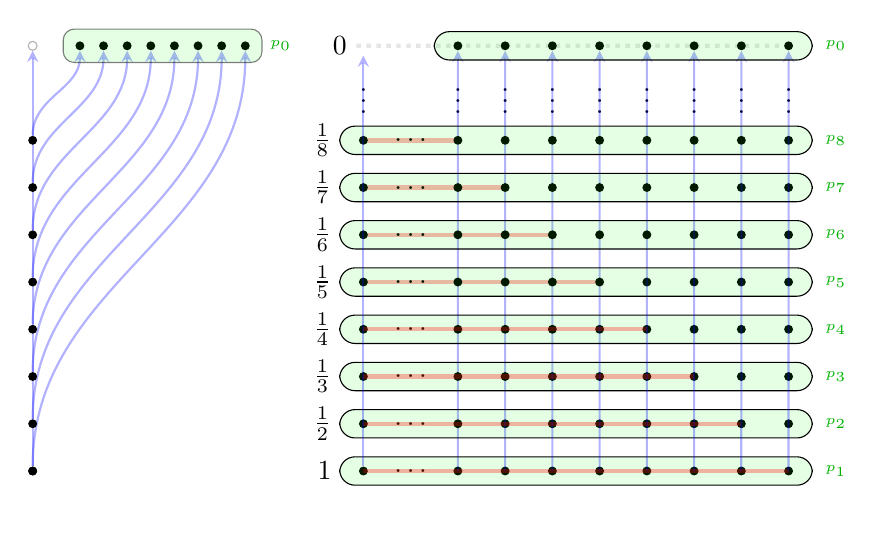
\begin{tikzpicture}[>=stealth, scale=.6,
world/.style={inner sep=.4mm, fill=black, circle},
intension/.style={fill=green, fill opacity=.1, rounded corners=5.5pt},
altrel/.style={->}]


%%%%%%%% SETTINGS %%%%%%%%%%%%%
\pgfmathtruncatemacro{\rows}{8}
\pgfmathsetmacro{\Dist}{-8}
%%%%%%%%%%%%%%%%%%%%%%%%%%%

\foreach \i in {1,2, ..., \rows}{
  \node[world](kicsi\i) at (-1,\i){};
  \node(pontok\i) at (0,\i){$\dots$};
 \foreach \j in {1,2, ..., \rows}{
  \node[world](\j\j) at (\j,\i){};
 }
  \draw[red, ultra thick, opacity=.3] (-1,\rows +1-\i)--(\i,\rows +1-\i);
  \node at (\i,\rows +1){$\vdots$};
  \node[world](veg\i) at (\i,\rows +2){};
  \draw[blue, thick, opacity=.3,altrel] (\i,1)--(veg\i);
\draw [intension] (-1.5,\i+.3) rectangle (\rows +.5,\i-.3);
\node[green!70!black] at (\rows+1,\i) {\tiny $p_\i $};
}

\node at (-1,\rows +1){$\vdots$};
\node (v1) at (-1.5,\rows +2) {$0$};
\node (v2) at (\rows,\rows +2) {};
\draw[ultra thick, opacity=.1, dotted]  (v1) edge (v2);
\node(nullavonal) at (-1,\rows +2) {};
\draw[blue, thick, opacity=.3,altrel] (kicsi1)--(nullavonal);

\node[anchor=east,inner sep=.4cm] at (kicsi1){$1$};
\foreach \i in {2, ..., \rows}{\node[anchor=east, inner sep=.4cm] at (kicsi\i){$\frac 1\i$};}

\draw [intension] (0.5,\rows+2.3) rectangle (\rows +.5,\rows+1.7);
\node[green!70!black] at (\rows+1,\rows+2) {\tiny $p_0$};

\begin{scope}[xshift= \Dist cm]
\node[world] (v3) at (0,1) {};
\node[world, fill=white, draw=black, opacity=.3] (v4) at (-0,10) {};
\draw[blue, thick, opacity=.3,altrel]  (v3) edge (v4);

\foreach \i in {1,2, ..., \rows}{
\node[world](w\i) at (0, \i){};
\node[world](v\i) at (1+0.5*\rows-.5*\i,\rows+2){};
\draw[blue, thick, opacity=.3,altrel] (w\i) edge[in=-90, out=90] (v\i);
}
\draw[intension, rounded corners=4pt, draw opacity=.5]  ([shift=(45:.5cm)]v1) rectangle ([shift=(225:.5cm)]v\rows);

\node[green!70!black] at (.5*\rows+1.25,\rows+2) {\tiny $p_0$};
\end{scope}
\end{tikzpicture}

\end{frame}
